\begin{enumerate}[1.]
\item Mark on a diagram the points $\brak{-2,4}, \brak{3,-5}$ and find the distance between them.

%
\item
Find the lengths of the lines joining the following pairs of points:
\begin{enumerate}
\item $\brak{-1,1}$ and $\brak{2,-1}$;
\item $\brak{4,3}$ and $\brak{-2,2}$;
\item \brak{a,b} and $\brak{-b,a}$.
\end{enumerate}

\item Prove that the line joining the points $\brak{2,1}$ and $\brak{4,7}$ has the same middle point as the line joining $\brak{5,4}$ and $\brak{1,4}$,
and hence that the four points are the corners of a parallelogram.
\item Prove that the points $\brak{-3,-4}, \brak{2,6}$ and $\brak{-6,10}$  are at the corners of a right-angled
traingle.
\item Plot the points $\brak{0,2},\brak{1,1},\brak{4,4}\text{ and }\brak{3,5}$ and prove that they are at the corners of a rectangle.
\item Plot the points $\brak{-2,-2},\brak{-1,2},\text{ and }\brak{3,1}$ and prove that they are at the corners of an isosceles triangle.
\item In the last question, find the distance of the vertex of the triangle from the middle point of the base.
\item Prove that the points $\brak{-1,0}$, $\brak{0,3}$, $\brak{3,2}$ and $\brak{2,-1}$ are at the corners of a square.
\item Prove that the points $\brak{-1,0}$, $\brak{3,1}$, $\brak{2,2}$  and $\brak{-2,1}$ are at the corners of a parallelogram. By finding
the coordinates verify that the joins of the middle points of pairs of opposite sides have the same middle point.
\item Prove that the points $\brak{21,-2}$, $\brak{15,10}$, $\brak{-5,0}$  and $\brak{1,-12}$ are at the corners of a rectangle, and find the
coordinates of its centre.
\item Find the lengths of the medians of the triangle whose corners are at the points $\brak{1,2}$, $\brak{0,3}$ and $\brak{-1,-2}$.
\item Find the coordinates of the points that divide the line joining the points $\brak{-35,-20}$ and $\brak{5,-10}$ into four equal parts.
\item Find the coordinates of the points of trisection of the line joining the points $\brak{-5,5}$ and $\brak{25,10}$.
\item Prove that the middle point of the line joining the points $\brak{-5,12}$ and $\brak{9,-2}$ is a point of trisection of the line
joining the points $\brak{-8,-5}$ and $\brak{7,10}$.
\item The points $\brak{8,5}$, $\brak{-7,-5}$ and $\brak{-5,5}$ are three of the corners of a parallelogram.  Find the coordinates of
the remaining corner which is to be taken as opposite to $\brak{-7,-5}$.
\item The point $\brak{2,6}$ is the intesection of the diagonals of a parallelogram two of whose corners are at the points $\brak{7,16}$ and $\brak{10,2}$.
Find the coordinates of the remaining corners.
\item Find the area of the triangle whose corners are the points $\brak{2,3}$, $\brak{-4,7}$ and $\brak{5,-2}$.  
\item Find the coordinates of  points which divide the join of $\brak{2,3}$, $\brak{-4,5}$ externally in the ratio $2:3$, and also
externally in the ratio $3:2$.
\item Prove that if $\brak{x_1,y_1},\brak{x_2,y_2}$ and $\brak{x_3,y_3}$ are the corners of a triangle the coordinates of its centroid are
\begin{equation*}
\frac{1}{2}\brak{x_1+x_2+x_3}, \frac{1}{2}\brak{y_1+y_2+y_3.}
\end{equation*}
\end{enumerate}
%\bibliography{IEEEabrv,gvv_opt}

%%\subsection{Driving the Segments}
\begin{problem}
Connect the $a-g$ pins of the display to the pins D2-D8 of the Arduino.
\end{problem}	
%
\begin{problem}
Open the arduino software.  Check if the ports show Arduino Uno and click the appropriate button.  
\end{problem}
\begin{problem}
\label{prob:first_code}
Type the following code and execute. What do you observe?
\lstinputlisting[language=C]{./codes/ard_dec_drive/src/main.cpp}
%// the setup function runs once when you press reset or power the board
int a=1,b=0,c=0,d=1,e=1,f=1,g=1;
void setup() {
    pinMode(2, OUTPUT);  
    pinMode(3, OUTPUT);
    pinMode(4, OUTPUT);
    pinMode(5, OUTPUT);
    pinMode(6, OUTPUT);
    pinMode(7, OUTPUT);
    pinMode(8, OUTPUT);            
}

// the loop function runs over and over again forever
void loop() {
  
  digitalWrite(2, a); 
  digitalWrite(3, b); 
  digitalWrite(4, c); 
  digitalWrite(5, d); 
  digitalWrite(6, e); 
  digitalWrite(7, f);     
  digitalWrite(8, g); 
}


\end{problem}
\begin{problem}
Now generate the numbers 0-9 by modifying the above program.
\end{problem}
%
%\newpage

%\section{Combinational Logic}
%
%\subsection{Counting Decoder}
%%
%\begin{problem}
%	\label{counter_dec}
%	In the  truth table in Table \ref{table:counter_decoder},  $W,X,Y,Z$ are the inputs
%and $A,B,C,D$ are the outputs. This table represents the system that increments the numbers 0-8 by 1 and resets the number 9 to 0
%%
%Note that  $D = 1$ for the inputs $0111$ and $1000$.  Using {\em boolean} logic,
%%
%\begin{equation}
%\label{bool_logic}
%D = WXYZ^{'} + W^{'}X^{'}Y^{'}Z
%\end{equation}
%%
%Note that $0111$ results in the expression $WXYZ^{'}$ and $1000$ yields $W^{'}X^{'}Y^{'}Z$. 
%
%Write the boolean logic functions for $A,B,C$ in terms of $W,X,Y,Z$.
%\end{problem}
%%
%\input{./figs/counter_decoder}
%The $\&\&$ operand is used for the boolean AND (multiplication) operation, the $||$ operand is used for the OR (addition) operation and the ! operand is used for the NOT ($^{'}$) operation in Arduino code.  For example, the expression for \eqref{bool_logic} in Arudino is
%\begin{verbatim}
%D = (W&&X&&Y&&!Z)||(!W&&!X&&!Y&&Z);
%\end{verbatim}
%%
%\begin{problem}
%Write the Arduino code for the outputs $A,B,C$ and verify if your logic is correct by observing the output on the seven segment display.
%\end{problem}
%%
%\subsection{Display Decoder}
%%
%\begin{problem}
%Now write the truth table for the seven segment display decoder (IC 7447).  The inputs will be $A,B,C,D$ and the outputs will be $a,b,c,d,e,f,g$.
%\end{problem}
%%
%\begin{problem}
%\label{seven_seg_disp_logic}
%Obtain the logic functions for outputs $a,b,c,d,e,f,g$ in terms of the inputs $A,B,C,D$.
%\end{problem}
%\begin{problem}
%Disconnect the arduino from IC 7447 and connect the pins D2-D8 in the Arduino directly to the seven segment display.
%\end{problem}
%\begin{problem}
%Write a new program to implement the logic in Problem \ref{seven_seg_disp_logic} and observe the output in the display.  You have designed the logic for IC 7447!
%\end{problem}
%\begin{problem}
%Now include your counting decoder program in the  display decoder program
%and see if the display shows the consecutive number.
%\end{problem}
%A decade counter counts the numbers from 0-9 and then resets to 0.
\begin{problem}
Suitably modify the above program to obtain a decade counter.
\end{problem}




%\begin{problem}
%Generate the boolean functions for the segments $a-f$ using the table in Problem \ref{bcd_ss}.  For example, the function for $a$ is obtained from the table as
%\begin{equation}
%a=\bar{D}\bar{C}\bar{B}A+\bar{D}C\bar{B}\bar{A}
%\label{boolean}
%\end{equation}
%\end{problem}
%%
%\begin{problem}
	%\label{counter_dec}
%Write functions for $A,B,C,D$ in Arduino using the following table and verify using the Arduino driven display.
		%\input{counter_decoder}
%\end{problem}
%\begin{problem}
	%Write a module for decimal to binary conversion
	%according to the example given below
	%\input{conversion}
	%%
	%$N \% 2$ gives the remainder and $N/2$ gives the quotient
%	and use it in the above code so that decimal values are given as input in the program and observed as output in the display. Note that the following code
%	\begin{verbatim}
%	a % b
%	\end{verbatim}
%	can be used to obtain the remainder when a is divided by b and
%	\begin{verbatim}
%	a/b
%	\end{verbatim}
%	gives the quotient.
%\end{problem}
 
%%
%\newpage
%\section{$M$-ary Modulation}
%\subsection{Angle Bisectors}

\begin{figure}[!ht]
	\begin{center}
		
		%
\includegraphics[width=\columnwidth]{./figs/ch3_angle_bisector}
		%\vspace*{-10cm}
		\resizebox{\columnwidth}{!}{\input{./figs/fig_3.0.tex}}
	\end{center}
	\caption{Angle bisectors meet at a point}
	\label{ch3_angle_bisector}	
\end{figure}

\begin{definition}
	In Fig. \ref{ch3_angle_bisector}, $OB$ divides the  $\angle B$ into half, i.e.\begin{equation}
	\angle OBC = \angle OBA
	\end{equation}
	$OB$ is known as an angle bisector.
\end{definition}
	$OB$ and $OC$ are angle bisectors of angles $B$ and $C$. $OA$ is joined and $OD, OF$ and $OE$ are perpendiculars to sides $a,b$ and $c$.
\begin{problem}
  Show that $OD = OE = OF$.
\end{problem}
\proof In $\Delta$s $ODC$ and $OEC$,
\begin{align}
OD &= OC \sin \frac{C}{2}
\\
OE &= OC \sin \frac{C}{2} 
\\
\Rightarrow OD &=OE.
\end{align}
Similarly,
\begin{equation}
OD = OF.
\end{equation}
%
\begin{problem}
	Show that OA is the angle bisector of $\angle A$
\end{problem}
\proof In $\Delta$s $OFA$ and $OEA$,
\begin{align}
OF &= OE
\\
\Rightarrow OA \sin OAF &= OA \sin OAE \\
\Rightarrow \sin OAF &=  \sin OAE \\
\Rightarrow \angle OAF &= \angle OAE
\end{align}
which proves that $OA$ bisects $\angle A$.
{\em Conclusion:} The angle bisectors of a triangle meet at a point.


\subsection{Congruent Triangles}
%
\begin{problem}
	Show that in $\Delta$s $ODC$ and $OEC$, corresponding sides and angles are equal.
\end{problem}
\begin{definition}
	Note that    $\Delta$s $ODC$ and $OEC$ are known as congruent triangles.  To show that two triangles are congruent, it is sufficient to show that some angles and sides are equal.
\end{definition}
\begin{problem}
SSS:	Show that if the corresponding sides of three triangles are equal, the triangles are congruent.
\end{problem}
\begin{problem}
ASA:	Show that if two angles and any one side  are equal in corresponding triangles, the triangles are congruent.
\end{problem}
\begin{problem}
SAS:	Show that if two sides and the angle between them are equal in corresponding triangles, the triangles are congruent.
\end{problem}
\begin{problem}
RHS:	For two right angled triangles, if the hypotenuse and one of the sides are equal, show that the triangles are congruent.
\end{problem}
	%
%%
\subsection{Perpendicular Bisectors}
\begin{definition}
	In Fig. \ref{ch3_perp_bisector}, OD $\perp BC$ and $BD=DC$. $OD$ is defined as the perpendicular bisector of $BC$.
\end{definition}

\begin{problem}
	In Fig. \ref{ch3_perp_bisector}, show that $OA=OB=OC$.
\end{problem}
%%
%%
\begin{figure}[!ht]
	\begin{center}
		
		\includegraphics[width=\columnwidth]{./figs/fig_3.8.eps}
%		
\includegraphics[width=\columnwidth]{./figs/ch3_perp_bisector}
		%\vspace*{-10cm}
%		\resizebox{\columnwidth}{!}{\input{./figs/fig_3.8.tex}}
	\end{center}
	\caption{Perpendicular bisectors meet at a point}
	\label{ch3_perp_bisector}	
\end{figure}
%
\proof In $\Delta$s $ODB$ and $ODC$, using Budhayana's theorem,
%
\begin{equation}
\begin{split}
OB^2 &= OD^2 + BD^2 \\
OC^2 &= OD^2 + DC^2 
\end{split}
\end{equation}
%
Since $BD = DC = \frac{a}{2}$, $OB = OC$.  Similarly, it can be shown that $OA = OC$.  Thus, $OA=OB=OC$.
%
\begin{definition}
	In $\Delta AOB$, $OA = OB$.  Such a triangle is known as an isoceles triangle.
\end{definition}
%
\begin{problem}
	Show that $AF = BF$.
\end{problem}
\proof Trivial using Budhayana's theorem.  This shows that $OF$ is a perpendicular bisector of $AB$. 
{\em Conclusion:}  The perpendicular bisectors of a triangle meet at a point.
%
\subsection{Perpendiculars from Vertex to Opposite Side}
	%
	%
	In Fig. \ref{ch3_perp_triang}, $AD \perp BC$ and $BE \perp AC$. $CF$ passes through $O$ and meets
	$AB$ at $F$.  	
\begin{problem}
	Show that 
	\begin{align}
	OE = c \cos A \cot C
	\end{align}
\end{problem}
	\begin{figure}[!ht]
		\begin{center}
			
			%
\includegraphics[width=\columnwidth]{./figs/ch3_perp_triang}
			%\vspace*{-10cm}
			\resizebox{\columnwidth}{!}{\input{./figs/fig_3.10.tex}}
		\end{center}
		\caption{Perpendiculars from vertex to opposite side meet at a point}
		\label{ch3_perp_triang}	
	\end{figure}
%
\proof In $\Delta$ s $AEB$ and $AEO$,
%
\begin{align}
AE &= c \cos A \\
OE &= AE \tan \brak{90^{\degree} - C} \brak{\because ADC \text{ is right angled}} \\
&= AE \cot C
\end{align}
%
From both the above, we get the desired result.
%
\begin{problem}
	Show that $\alpha = A$.
\end{problem}
\proof In $\Delta OEC$,
%
\begin{equation}
CE = a \cos C \brak{\because BEC \text{ is right angled}}
\end{equation}
%
Hence,
%
\begin{equation}
\begin{split}
\tan \alpha &= \frac{CE}{OE} \\
&=  \frac{a \cos C}{c \cos A \cot C} \\
&=  \frac{a \cos C \sin C}{c \cos A \cos C} \\
&= \frac{a \sin C}{c \cos A } \\
&= \frac{c \sin A}{c \cos A } \brak{\because \frac{a}{\sin A} = \frac{c}{\sin C}}\\
&= \tan A\\
\Rightarrow \alpha = A
\end{split}
\end{equation}
%
\begin{problem}
	Show that $CF \perp AB$
\end{problem}
\proof Consider triangle OFB and the result of the previous problem.  $\because$ the sum of the angles of a triangle is $180^{\degree}$, $\angle CFB = 90^{\degree}$.
{\em Conclusion: The perperdiculars from the vertex of a triangle to the opposite side meet at a point.} 
%
%\newpage
%\section{BER in Rayleigh Flat Slowly Fading Channels}
	%\subsection{Chord of a Circle}
%
\renewcommand{\theequation}{\theenumi}
\begin{enumerate}[label=\arabic*.,ref=\thesubsection.\theenumi]
\numberwithin{equation}{enumi}
%
\item
	Fig. \ref{ch4_circle_def} represents a circle.  The points in the circle are at a distance $r$ from the centre $O$.  $r$ is known as the radius.

\begin{figure}[!ht]
	\begin{center}
		
		%
\includegraphics[width=\columnwidth]{./figs/ch4_circle_def}
		%\vspace*{-10cm}
		\resizebox{\columnwidth}{!}{\input{./figs/fig_4.0.tex}}
	\end{center}
	\caption{Circle Definitions}
	\label{ch4_circle_def}	
\end{figure}
\end{enumerate}
\subsection{Chords of a circle}
%
\renewcommand{\theequation}{\theenumi}
\begin{enumerate}[label=\arabic*.,ref=\thesubsection.\theenumi]
\numberwithin{equation}{enumi}
%
\item
	In Fig. \ref{ch4_circle_def}, $A$ and $B$ are points on the circle.  The line $AB$ is known as a chord of the circle.

%
%
\item
	\label{ch4_prob_circle_subtend}
	In Fig. \ref{ch4_circle_subtend}  Show that $\angle AOB = 2\angle ACB $.

\begin{figure}[!ht]
	\begin{center}
		
		%
\includegraphics[width=\columnwidth]{./figs/ch4_circle_subtend}
		%\vspace*{-10cm}
		\resizebox{\columnwidth}{!}{\input{./figs/fig_4.1.tex}}
	\end{center}
	\caption{Angle subtended by chord $AB$ at the centre $O$ is twice the angle subtended at $P$. }
	\label{ch4_circle_subtend}	
\end{figure}

\solution In Fig. \ref{ch4_circle_subtend}, the triangeles $OPA$ and $OPB$ are isosceles. Hence,
%
\begin{align}
\angle OCA = \angle OAC &= \theta_1 \\
\angle OCB = \angle OBC &= \theta_2
\end{align}
%
Also, $\alpha$ and $\beta$ are exterior angles corresponding to the triangle $AOC$ and $BOC$ respectively. Hence
%
\begin{align}
\alpha &= 2\theta_1 \\
\beta &= 2\theta_2
\end{align}
%
Thus,
%
\begin{align}
\angle AOB &= \alpha + \beta \\
&= 2\brak{\theta_1 + \theta_2} \\
&= 2\angle ACB
\end{align}
%
\item
	The diameter of a circle is the chord that divides the circle into two equal parts. In Fig. \ref{ch4_circle_dia}, $AB$ is the diameter and passes through the centre $O$

%
\item
In Fig. \ref{ch4_circle_dia}, show that $\angle APB = 90^{\degree}$ .

%
\begin{figure}[!ht]
	\begin{center}
		
		%
\includegraphics[width=\columnwidth]{./figs/ch4_circle_dia}
		%\vspace*{-10cm}
		\resizebox{\columnwidth}{!}{\input{./figs/fig_4.2.tex}}
	\end{center}
	\caption{Diameter of a circle.}
	\label{ch4_circle_dia}	
\end{figure}
\item
	In Fig. \ref{ch4_chord_product}, show that 
	\begin{equation}
	\begin{split}
\angle ABD &= \angle ACD \\
\angle CAB &= \angle CDB	
	\end{split}
	\end{equation}

\begin{figure}[!ht]
	\begin{center}
		
		%
\includegraphics[width=\columnwidth]{./figs/ch4_chord_product}
		%\vspace*{-10cm}
		\resizebox{\columnwidth}{!}{\input{./figs/fig_4.3.tex}}
	\end{center}
	\caption{$PA.PB = PC.PD$}
	\label{ch4_chord_product}	
\end{figure}
%
%
\solution Use Problem \ref{ch4_prob_circle_subtend}.
%
\item
	In Fig. \ref{ch4_chord_product}, show that the triangles $PAB$ and $PBD$ are similar

\solution Trivial using previous problem
\item
	In Fig. \ref{ch4_chord_product}, show that 
	\begin{equation}
	PA.PB = PC.PD
	\end{equation}

%
\solution Since triangles $PAC$ and $PBD$ are similar, 
%
\begin{align}
\frac{PA}{PD} &= \frac{PC}{PB} \\
\Rightarrow PA.PB &= PC.PD
\end{align}
%
%
\item
	Show that 
	\begin{equation}
	\label{ch5_sin_zero}
	\sin 0^{\degree} = 0
	\end{equation}

\solution Follows from \eqref{ch5_sin_increasing}.
%
\item
	Show that 
	\begin{equation}
	\label{ch5_sin_zero}
	\cos 0^{\degree} = 1
	\end{equation}
	
\item
	The line $PX$ in Fig. \ref{ch4_tangent_def} touches the circle at exactly one  point $P$. It is known as the tangent to the circle.

%
%
\item
	Show that $OP \perp PX$.
% is the perpendicular to the line $PX$ as shown in the Fig. \ref{ch4_short_dist}. Show that $OP$ is the shortest distance between the point $O$ and the line $PX$. 

\solution Without loss of generality, let $0 \le \theta \le 90^{\degree}$. Using the cosine formula in $\triangle OPP_n$,\begin{align}
\brak{r+d_n}^2 > r^2,
\end{align}
%Let $P_1$ be a point on the line $PX$. Then $OPP_1$ is a right angled triangle.  Using Budhayana's theorem,
%
\begin{figure}[!ht]
	\begin{center}
		
		%
\includegraphics[width=\columnwidth]{./figs/ch4_tangent_def}
		%\vspace*{-10cm}
		\resizebox{\columnwidth}{!}{\begin{tikzpicture}
[scale =2,>=stealth,point/.style = {draw, circle, fill = black, inner sep = 1pt},]

\def\rad{2}
\coordinate [point, label={right: $O$ }] (O) at (0, 2);
\draw (O) circle (\rad);
\node (P) at (0,0)[point,label=below :$P$] {};
\node (X) at (2,0)[point,label=right :$X$] {};
\node (Y) at (-4,0)[point,label=left :$Y$] {};
\node (P_1) at (-1,0)[point,label=below  :$P_1$] {};
\node (P_2) at (-2,0)[point,label=below  :$P_2$] {};
\node (P_3) at (-3,0)[point,label=below  :$P_3$] {};

\draw (O)--(P);
\draw (X)--(Y);
\draw (O)--(P_1);
\draw (O)--(P_2);
\draw (O)--(P_3);

\tkzMarkRightAngle[size=.2](O,P,P_1);
\node [above] at (-0.8,0.5){$r$};
\node [above] at (-1.2,0.8){$r$};
\node [above] at (-1.45,1){$r$};
\node [above] at (0.1,0.8){$r$};
\end{tikzpicture}}
	\end{center}
	\caption{Tangent to a Circle.}
	\label{ch4_tangent_def}	
\end{figure}
%
%\begin{figure}[!ht]
%	\begin{center}
%		
%		%
\includegraphics[width=\columnwidth]{./figs/ch4_short_dist}
%		%\vspace*{-10cm}
%		\resizebox{\columnwidth}{!}{\input{./figs/fig_4.6_1.tex}}
%	\end{center}
%	\caption{Shortest distance from $O$ to line $PX$}
%	\label{ch4_short_dist}	
%\end{figure}

%
\begin{align}
%\begin{split}
\brak{r+d_n}^2 = r^2 + x_n^2 - 2rx_n\cos\theta > r^2 
\\
\implies  0 <\cos\theta < \frac{x_n}{2r},
%OP_1^2 &= OP^2 + PP_1^2 \\
%\Rightarrow OP_1 > OP
%\end{split}
\end{align}
%
where $x_n$ can be made as small as we choose.  Thus, 
%
\begin{align}
\cos \theta = 0 \implies \theta  = 90 ^{\degree}.
\end{align}

%\solution In Fig. \ref{ch4_tangent_def}, we can see that $OP$ is is the radius of the circle and the length of all line segments from $O$ to the line $PX > r$.  Using the result of the previous 
%problem, it is obvious that $OP \perp PX$. 
%
	%
\item
In Fig. \ref{ch4_tangent_prod} show that 
%
\begin{equation}
\angle PCA = \angle PBC
\end{equation}
%
$O$ is the centre of the circle and $PC$ is the tangent.

	\begin{figure}[!ht]
		\begin{center}
			
			%
\includegraphics[width=\columnwidth]{./figs/ch4_tangent_prod}
			%\vspace*{-10cm}
			\resizebox{\columnwidth}{!}{\input{./figs/fig_4.8.tex}}
		\end{center}
		\caption{$PA.PB = PC^2$.}
		\label{ch4_tangent_prod}	
	\end{figure}
	%

%
\solution Obvious from the figure once we observe that $\triangle OAC$ is isosceles.
%
%
\item
	In Fig. \ref{ch4_tangent_prod}, show that the triangles $PAC$ and $PBC$ are similar.

\solution From the previous problem, it is obvious that corresponding angles of both triangles are equal.  Hence they are similar.
%
\item
	Show that $PA.PB = PC^2$

\solution Since $\Delta PAC \sim \Delta PBC$, their sides are in the same ratio.  Hence,
%
\begin{align}
\frac{PA}{PC} &= \frac{PC}{PB} \\
\Rightarrow PA.PB &=PC^2
\end{align}
%
\item
Given that $PA.PB = PC^2$, show that $PC$ is a tangent to the circle.

%
\item
	In Fig. \ref{ch4_chord_tangent_prod}, show that\begin{equation}
	PA.PB = PC.PD
	\end{equation}

%
\begin{figure}[!ht]
	\begin{center}
		
		%
\includegraphics[width=\columnwidth]{./figs/ch4_chord_tangent_prod}
		%\vspace*{-10cm}
		\resizebox{\columnwidth}{!}{\input{./figs/fig_4.11.tex}}
	\end{center}
	\caption{$PA.PB = PC^2$.}
	\label{ch4_chord_tangent_prod}	
\end{figure}

\solution Draw a tangent and use the previous problem.
\end{enumerate}
 




